\documentclass[cacheSimReport.tex]{subfiles}
\begin{document}

\section*{\textsc{\Large Results and Discussion}}

The first valuable metric is a comparison of the execution times between the different traces as well as the different configurations.

\smallskip

\hspace{-.9cm}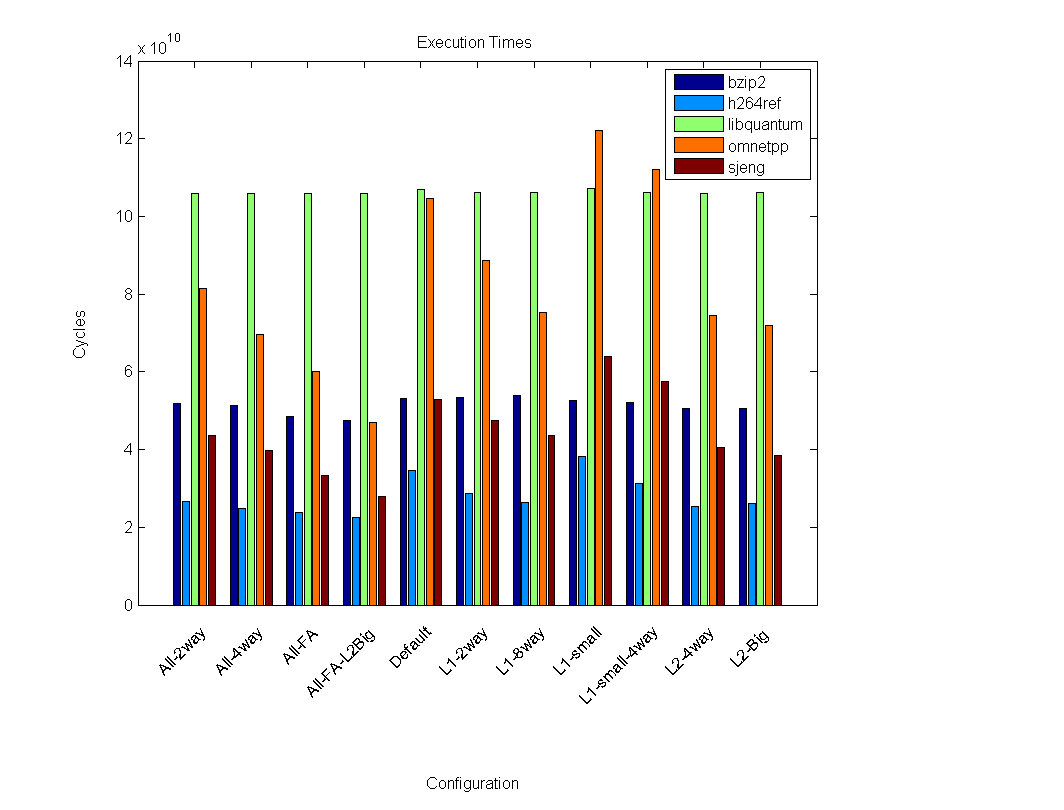
\includegraphics{executionTime.png}

In this figure the columns of the bar chart are organized first by the configuration run, then the trace. Excepting the libquantum trace, the traces follow a regular pattern. The execution times go from smallest with the All-FA-L2Big configuration to the largest execution time L1-small. The amount of variation for different traces also differs greatly. Libquantum and bzip2 have a relatively small amount of variation between different configs, while omnetpp varies wildly. This behavior is likely due to the types of instructions contined within the trace. The omnetpp trace, for example, gains large benifits from increasing the associativity of both the L1 and L2 cache, as well as benefit from increasing the size of the L2 cache. The libquantum trace acts in a different fashion, not seeming to gain benefit from any sort of modifications made to the cache structure. Though libquatum was the smallest trace size at 4.2GB, it took the most cycles to run in 9 of the 11 configurations this is likely due to its hit rate which will be discussed later in this section.

\smallskip

The next five images show comparisons of the hit rates for the L1 caches and the L2 cache for each of the different configurations with each of the five traces. This data sheds light on the results in the previous section.

\hspace{-.9cm}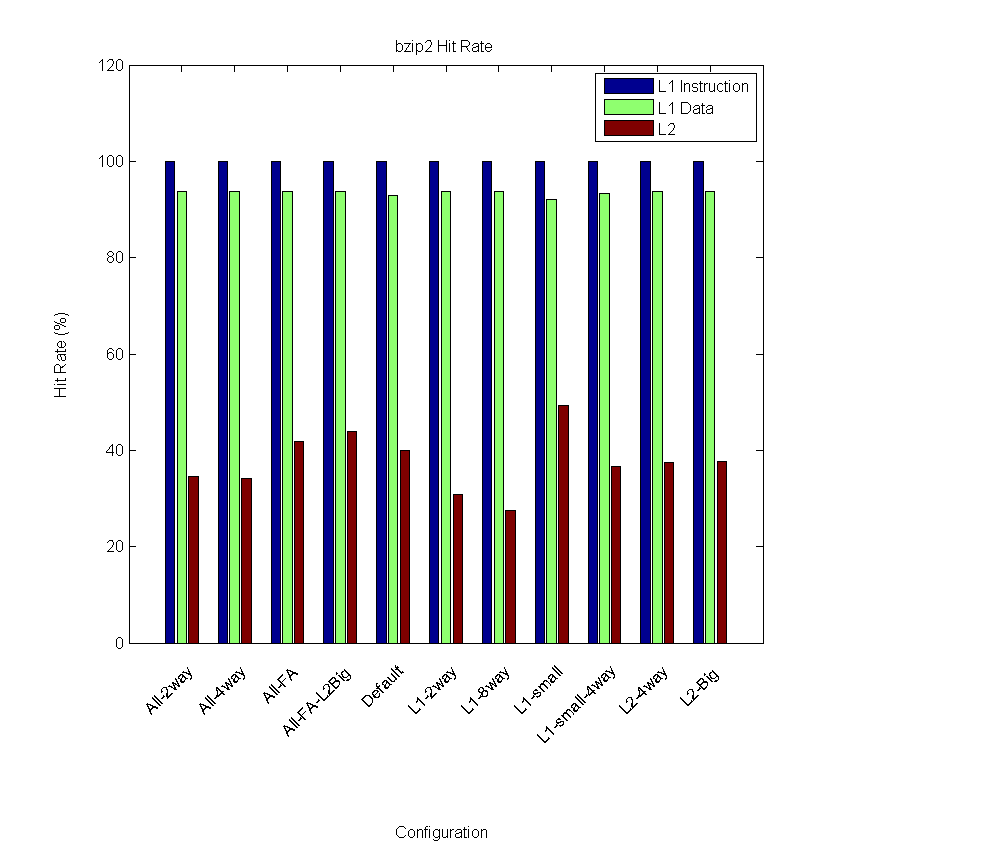
\includegraphics{hitRate_bzip2.png}

The hit rate results are different for the bzip2 trace as they have by far the lowest L2 cache hit rate at every configuration. The L1 instruction hit rate is near 100\% while the L2 data hit rate hovers at around 93\%. These relatively good hit rates keep the run time on the low side, but the under 50\% L2 hit rate takes a toll on overall performance.

\hspace{-.9cm}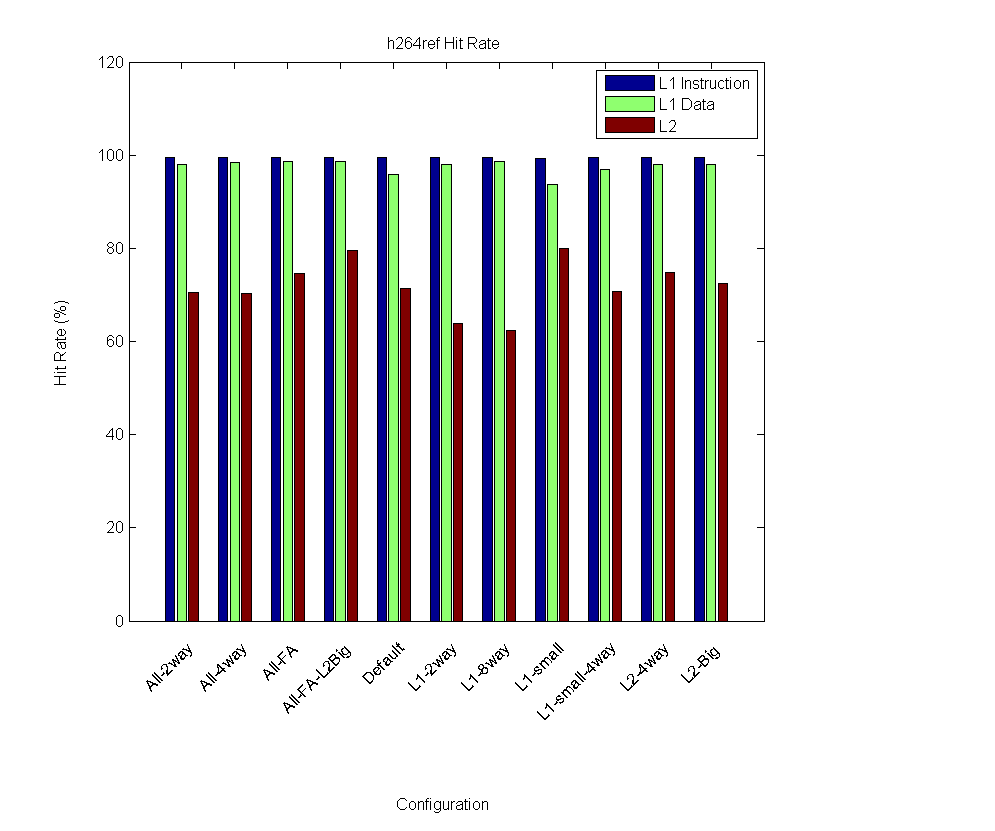
\includegraphics{hitRate_h264ref.png}

The h264ref trace had the best performace out of any trace at each of the different configurations. This makes some sense as it is the second smallest trace at 4.7GB, and therefore has fewer total references than the bigger traces. Only the libquantum traces is smaller, and it has other performance issues. The hit rate for the L1 instruction cache is near 100\% for each of the configurations. The L1 data cache also consitently performes better than the rest of the traces. the h264ref trace additionally has a relatively good L2 hit rate whcih increases dramatically when the L2 cache is fully associative.

\hspace{-.9cm}\includegraphics{hitrate_libquantum.png}

The libquantum trace had the most unusual characteristics. Though it was a small trace as discussed earlier, it took the most cycles to execute through the majority of the trials. The reason the exection time is so much longer has to do with the read instructions. Only 21.4\% of the references were reads, but they took up 81.9\% of the total execution time averaging 24.9 cycles per read instruction. Meanwhile, many of the other traces such as the sjeng trace have a smaller percentage of read instructions as well as a CPI of under 10. Another oddity with the libquantum trace is that for the different configurations, all of the exection times as well as the hit and miss rates were are near exactly the same. It is the only trace to exhibit this behavior. The trace that acts most similarly, bzip2, shares the characteristic of a low L2 cache hit rate, but libquantum's hit rate is not nearly as low. 

\hspace{-.9cm}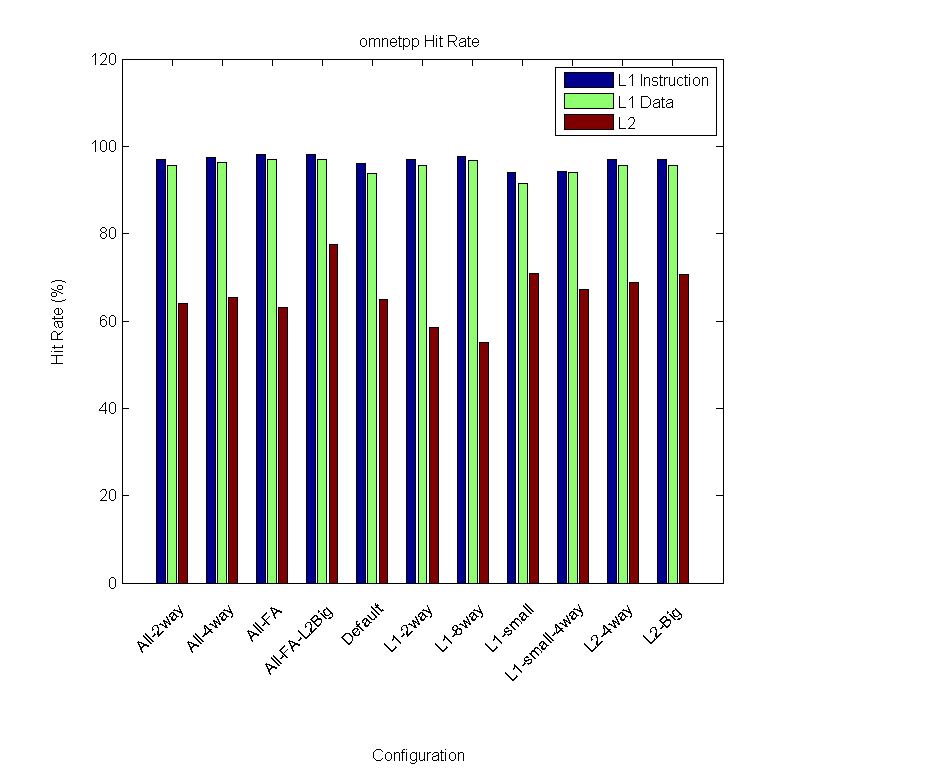
\includegraphics{hitRate_omnetpp.png}

The omnetpp trace had the most variety in exection time. This is likely due to its lower than average L1i hit rate. Most traces are near 100\% on the L1i hit rate, but the omnetpp hit rate is slightly lower, this means that more requests are going to L2 so a bigger or more associative L2 cache contributes greatly to the performance of the trace overall.

\hspace{-.9cm}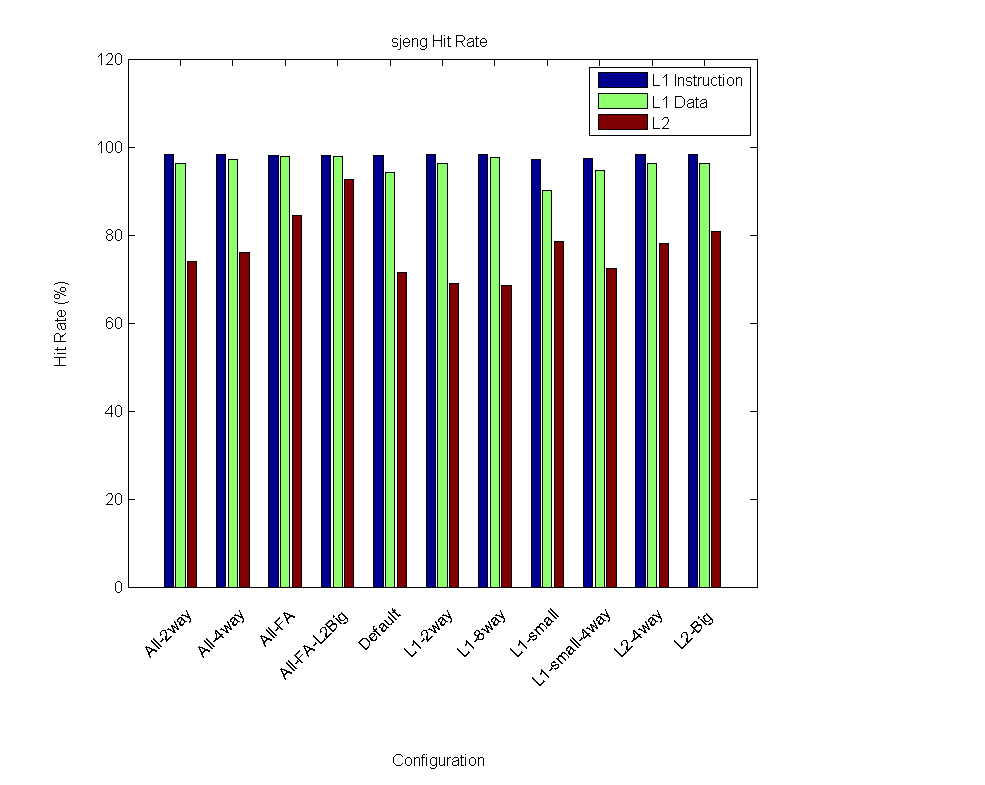
\includegraphics{hitRate_sjeng.png}
 
The sjeng trace has the highest average L2 hit rate of any of the traces in the ALL-FA-L2Big configuration at 92.6\%, this is the only L2 hit rate that goes above 90\% for any of the traces or configurations. This likely has to do with the relative consistency of the types of instructions. Even if the reference does not hit in the L1 caches, the odds are better for it hitting in the L2 if the references vary less.

\smallskip

The next two images deals again with the sjeng trace, but in this case the default configuration was used and the chunk size was modified. The chunk size comes into play during L2 misses. It defines the amount of information that can be carried from memory to the L2 cache at a time.

\hspace{-.9cm}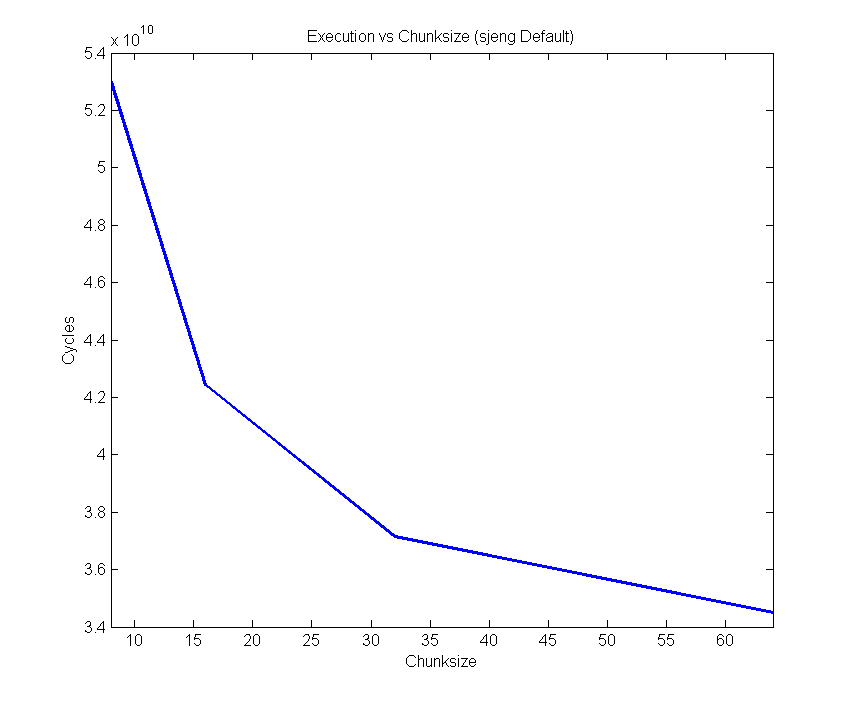
\includegraphics{chunksizeExecution.png}

The default chunksize is 8 bytes. This takes around 53 billion cycles to perform. At the maximum chunk size, 64 bytes, the execution time goes down to 34.5 billion cycles. As the chunk size continues to increase, the effectiveness of each doubling goes down substatially. The increase from an 8 byte chunk size to a 16 byte chunk size is almost as large as the gap between a 16 byte chunk size and a 64 byte chunk size.

\hspace{-.9cm}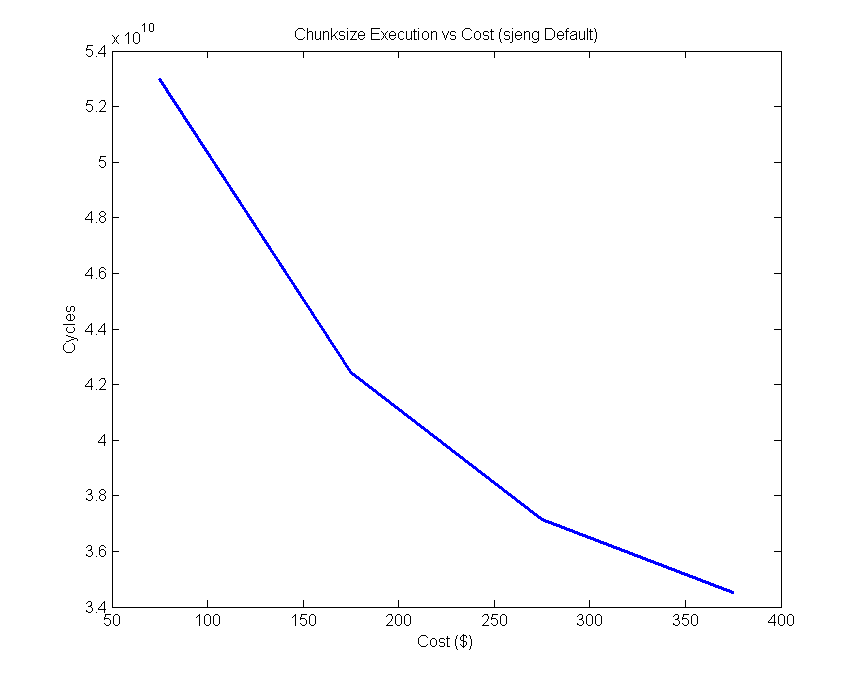
\includegraphics{chunksizeExecutionVsCost.png}

The next logical step is comparing the execution with the new chunksizes to the cost of the memory model. The cost graph is closer to linear than execution curve. A steeper slope on this graph is suggests a more efficieny in the system per dollar. Again the first doubling of the chunk size grants more utility than later doublings.

\smallskip

The final two images compare the costs of the different configurations and their speed. 

\hspace{-.9cm}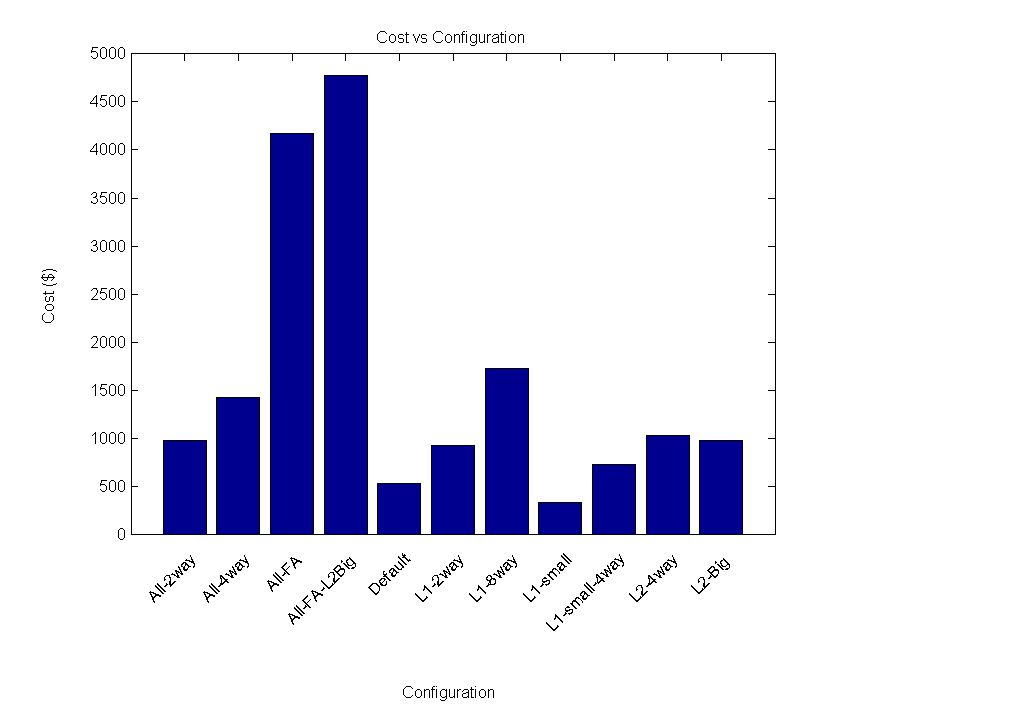
\includegraphics{costVsConfiguration.png}

This figure clearly shows that making caches fully associative is incredibly expensive. Other modifications increase the price from default, but the expanding a system to fully associative comes with incredible cost.

\hspace{.9cm}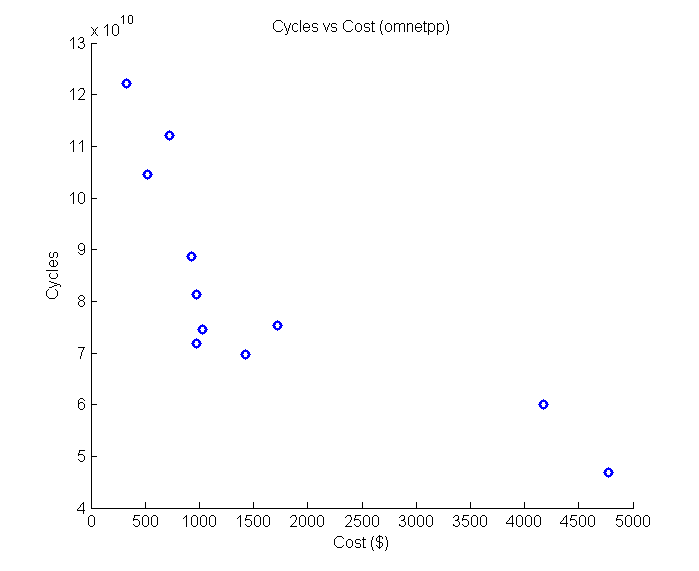
\includegraphics{cyclesVsCost.png}

The plot in this image is a good place to start for choosing an optimal configuration. The trace used in this image is the omnetpp trace. It was chosen because it showed the greatest desparity in execution time for the different configurations, for this reason it highights the best choice in this scenario. The point with the lowest distance from the origin would be the most efficient implementation for the cost. In this case that point represents the L2-Big configuration.

\smallskip

The final two figures expand on the idea in the previous sectino in order to come to a conclusion about which configuration is more efficient on the whole. The total cycles are averaged for each configuration.

\hspace{-.9cm}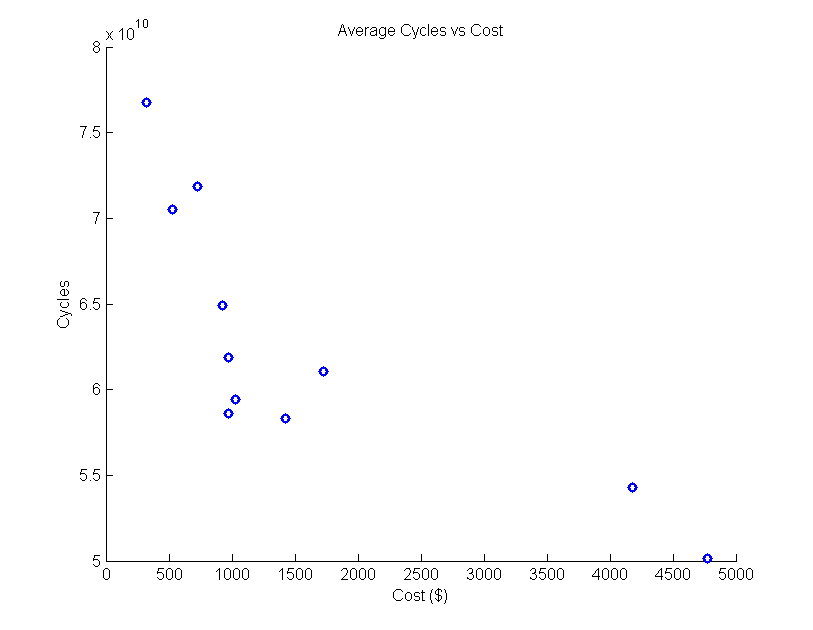
\includegraphics{averageCyclesVsCost.png}

This figure shows a similar image to the scatter plot used for the omnetpp trace. This time the figure includes every trace. None the less it looks very similar. This is due to all of the traces following similar patterns in execution time for the different traces. Again the L2-Big configuration is closest to the origin, meaning that it is the most effieicnt configuration for the traces at hand.

\hspace{.9cm}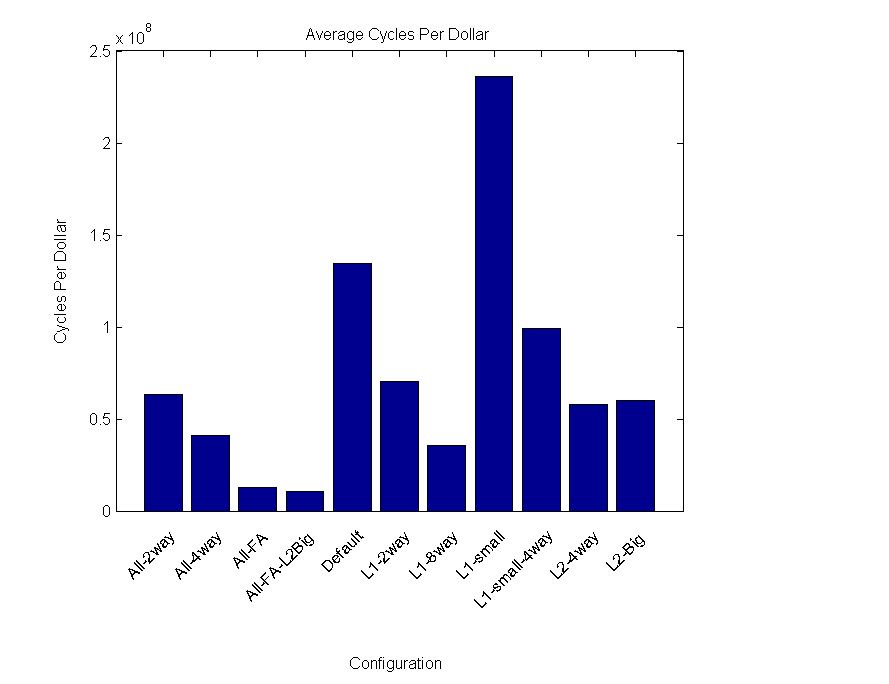
\includegraphics{averageCyclesPerDollar.png}

This chart quantifies the optimization by plotting cycles vs cost. This plot is better for showing cost constraints. if the budget for the system is very very low, the L1-small trace does a good job of using each dollar very efficiently. The fully associtive traces on the other hand get very few cycles per dollar.


\end{document}